\chapter{実装}
{
\label{chap:implement}
本章では\ref{chap:parallel}章の並列化に対する検討を元にして、FPGAに実装するアクセラレータについて解説する。
\section{スレッド並列化の実装}
\label{sec:thread_impl}
図\ref{fig:para_inception}で示した4つの計算スレッドについて、各スレッドにそれぞれ1枚のFPGAで演算を行うようにする。

\section{スレッド内モジュールの実装}
\label{sec:module_impl}
FiCのマルチFPGAシステムでは、流れてきたデータをそれぞれのFPGAボードでの処理を終えて、次のFPGAに出力を渡す、というフローが想定される。
そのため各ボードでは特定の演算処理のみを実行すればよいので\cite{optimized}のように複数のサイズの畳み込みを行うことは考えずに、
それぞれの層に適した入出力サイズのモジュールを実装することが可能である。また特定の層の重みフィルタのみをBRAMに保存して読み出し演算を行う。
各スレッドのモジュールはまず、ブロードキャストされる同一サイズの入力値を受け取る。その後、BRAMの重みフィルタとの畳み込み演算を行う。
図\ref{fig:thread_module}にモジュールの模式図を示す。
\begin{figure}[h]
    \centering
    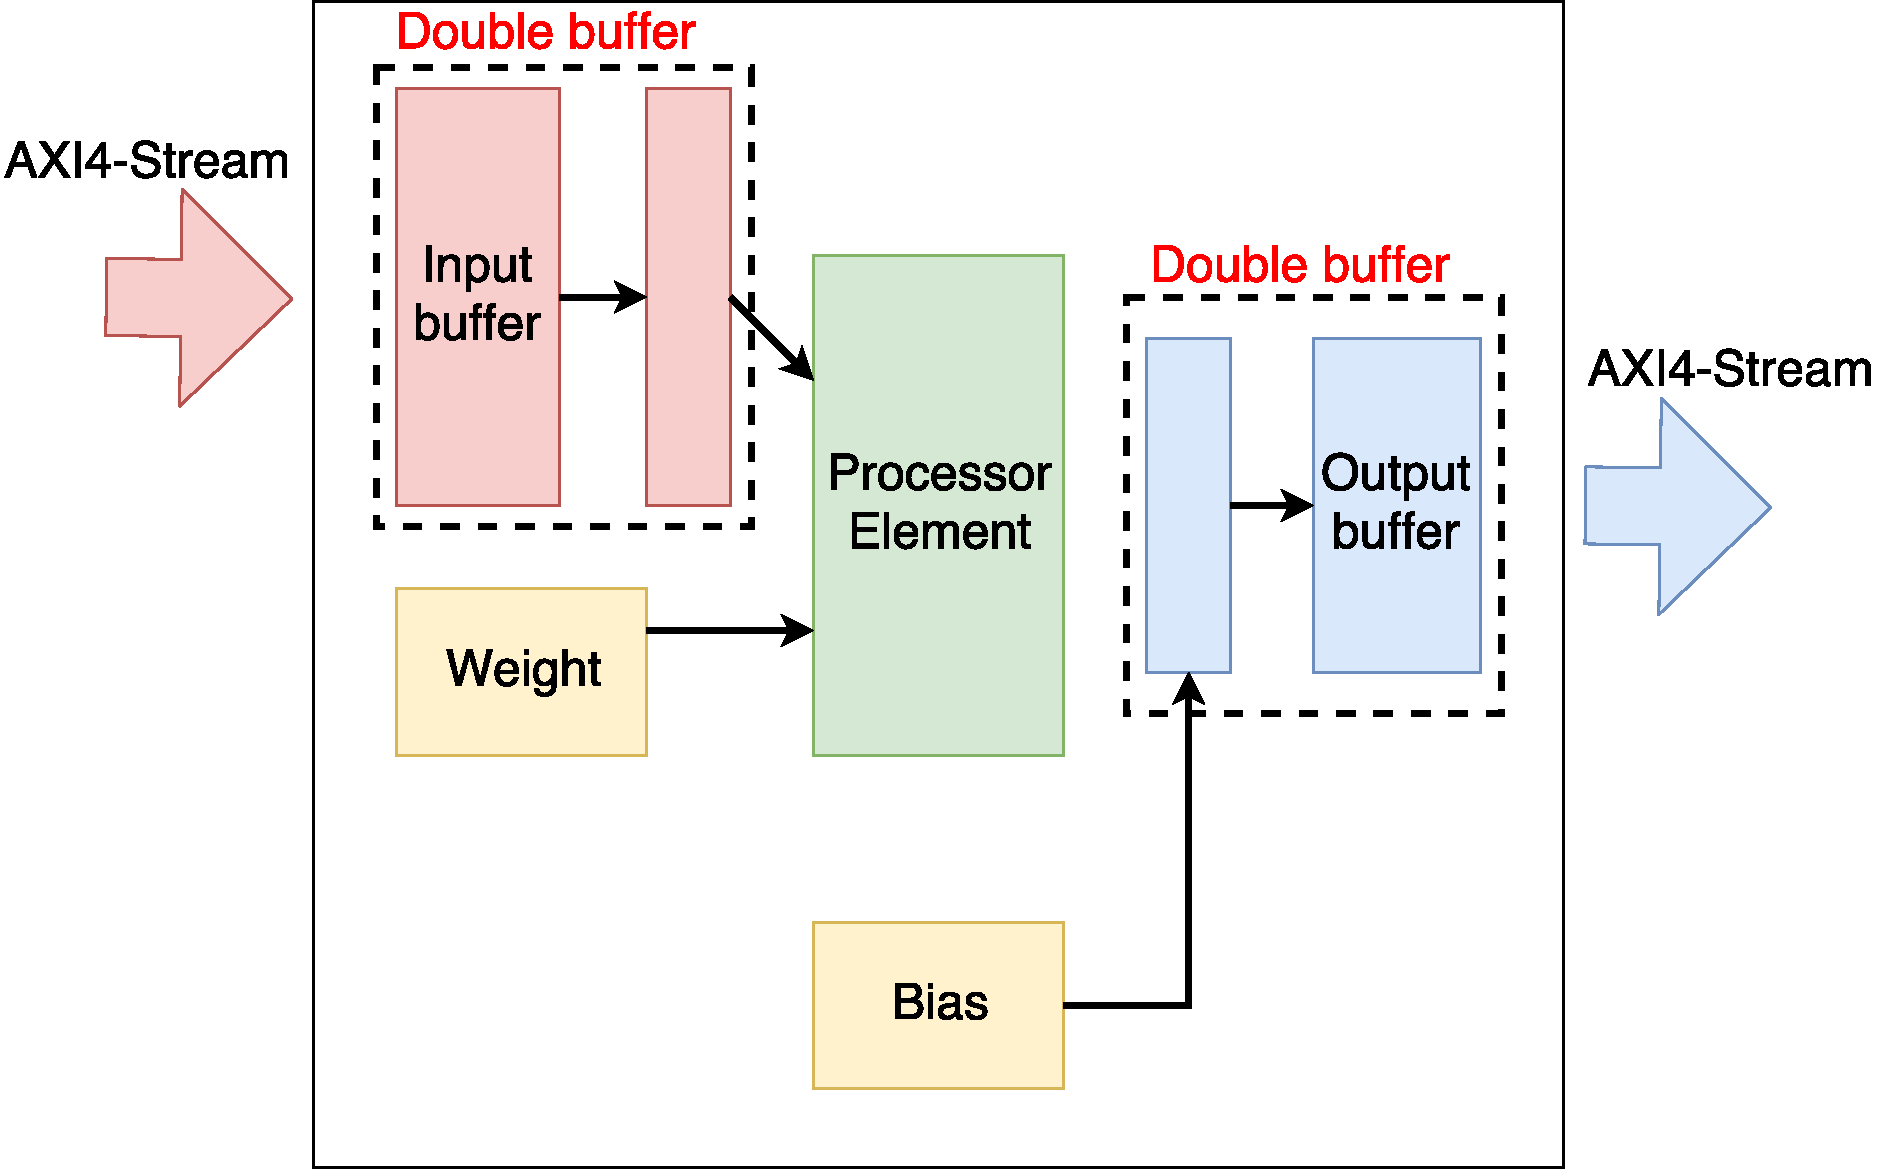
\includegraphics[width=12cm]{./chap6/fig/thread_module.pdf}
    \caption{モジュールの模式図}
    \label{fig:thread_module}
\end{figure}
入出力のインターフェイスにはXilinxが提供するAXI4-Streamを利用する。
AXI4-Streamはデータストリーム用のインターフェイスである。これにより入出力データをストリーム形式で送受信できる。
図\ref{fig:thread_module}に示すように入出力、重みフィルタにダブルバッファを設けることで演算に必要なデータを受け取ったら、
演算を行うと同時にもう片方のバッファで次のデータの書き込みが可能となる。

畳み込み演算はPEで行う。図\ref{fig:para_inception}で示した4つの計算スレッドのうちthread2、thread3、thread4については畳み込みやpooling処理
が連続して行われているので図\ref{fig:thread_module}が2つ接続するようなモジュールとなる。

\section{畳み込み演算器の実装}
\label{sec:conv_impl}
\ref{sec:module_impl}節で述べたモジュールの模式図内のPE部の設計は\cite{optimized}を参考にした。
ここでは\ref{code:conv}に示す、畳み込み演算のCコードをループタイリングによって分割することで並列化することを考える。

\begin{itembox}[1]{畳み込み演算のCコード}
    \label{code:conv}
    \begin{verbatim}
    for (int r = 0; r < R; r++)
      for (int c = 0; c < C; c++)
        for (int to = 0; to < M; to++)
          for (int ti = 0; ti < N; ti++)
            for (int i = 0; i < K; i++)
              for (int j = 0; j < K; j++)
                output[to][r][c] +=
                  input[ti][S*r+i][S*c+j] *
                  weight[to][ti][i][j];
    \end{verbatim}
\end{itembox}

\begin{itembox}[1]{出力特徴マップチャンネルで並列化された畳み込み演算のCコード}
    \
    \begin{verbatim}
    for (int r = 0; r < R; r++)
      for (int c = 0; c < C; c++)
        for (int to = 0; to < M; to += Tm) //Tmごとに出力を分割
          for (int ti = 0; ti < N; ti++)
            for (int i = 0; i < K; i++)
              for (int j = 0; j < K; j++)
                output[to][r][c] +=
                  input[ti][S*r+i][S*c+j] *
                  weight[to][ti][i][j];
    \end{verbatim}
\end{itembox}

\ref{code:conv_tile}がループタイリングを行った疑似コードである。$T_m$、$T_n$がそれぞれ入力値、出力値のタイルのサイズとなっている。
この疑似コードに倣って演算モジュールを作ると図\ref{fig:conv_pe}のような演算器を設計できる。

\begin{figure}[h]
    \centering
    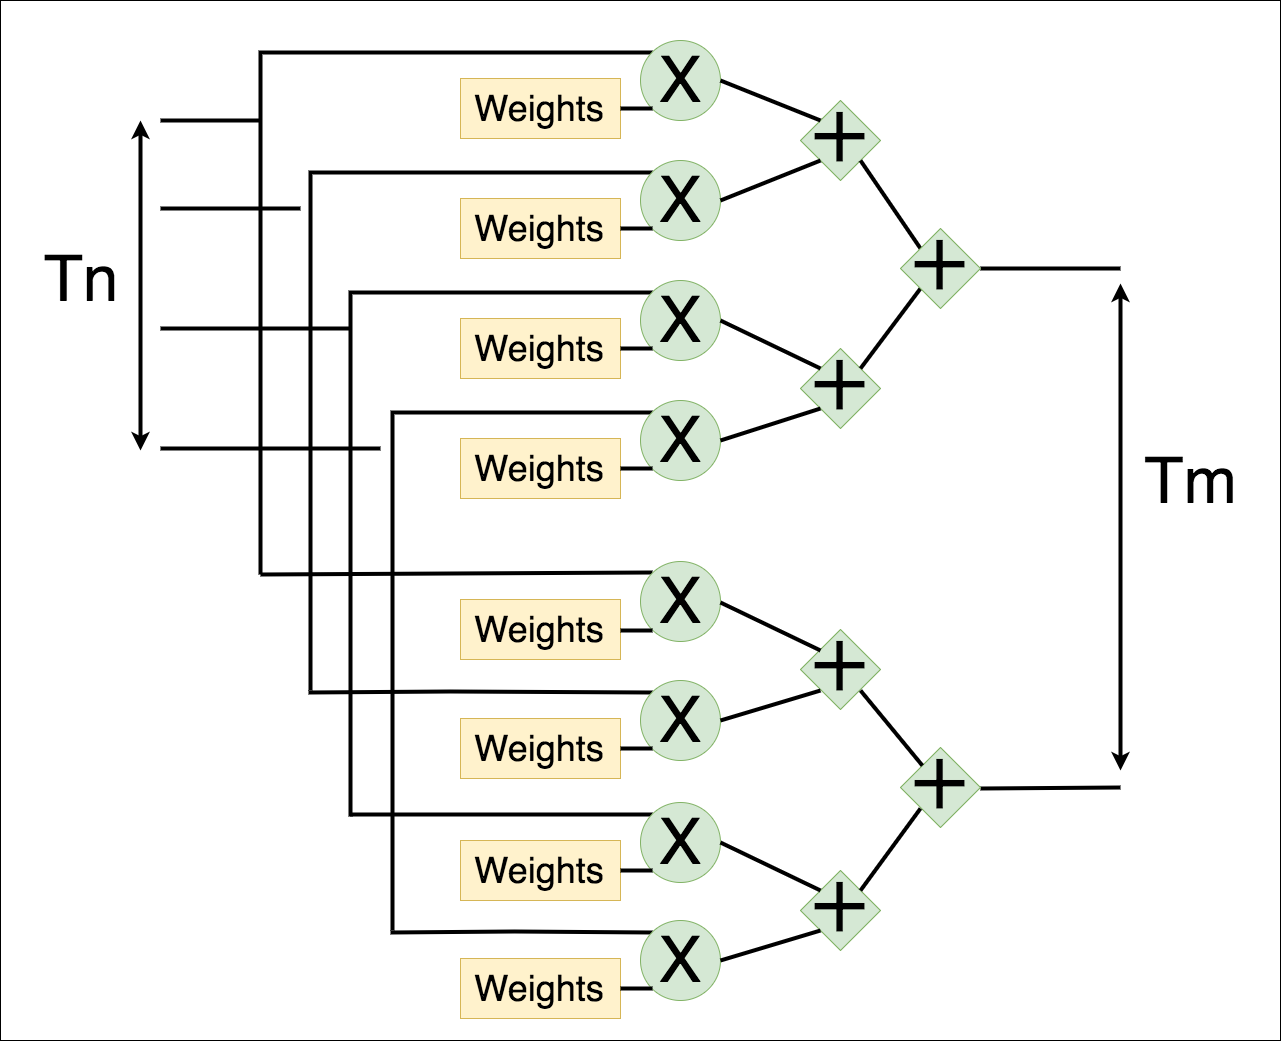
\includegraphics[width=12cm]{./chap6/fig/ucla_pe.png}
    \caption{畳み込み演算器の模式図}
    \label{fig:para_inception}
\end{figure}
% 畳み込み演算器のタイリングしたモジュールの説明を入れる。
}

